\documentclass[letter,12pt]{article}

\newcommand{\blind}{1}
\newcommand{\georddtitle}{
    A Bayesian Nonparametric Approach to Geographic Regression Discontinuity Designs:
    Do School Districts Affect NYC House Prices? \\*
    ~\\*
    Supplementary Materials
}
% Nicer default font (+ math font) than Computer Modern for most use cases
\usepackage{mathrsfs}
\usepackage{graphicx}
\usepackage{xr-hyper} % cross-references (between documents)
\usepackage{xcolor} % Allow colors to be defined
\usepackage{geometry} % Used to adjust the document margins
\usepackage{amsmath} % Equations
\usepackage{amssymb} % Equations
% The hyperref package gives us a pdf with properly built
% internal navigation ('pdf bookmarks' for the table of contents,
% internal cross-reference links, web links for URLs, etc.)
\usepackage[hyphens]{url}
\usepackage[hypertexnames=false]{hyperref}
\usepackage[title,toc]{appendix}
\newcommand{\georddtitle}{
    A Bayesian Nonparametric Approach to Geographic Regression Discontinuity Designs:
    Do School Districts Affect NYC House Prices?
}
\hypersetup{
    colorlinks=true,
    pdfborder=0 0 1,
    pdftitle=\georddtitle{},
    allcolors=[rgb]{0.00,0.38,0.59},
    allbordercolors=[rgb]{0.60,0.76,0.86}
}
\usepackage{natbib}
\usepackage{bm}
\usepackage{mathtools}
\usepackage{pdflscape}
\usepackage[nodisplayskipstretch]{setspace}
% only use if doublespacing:
\renewcommand*{\arraystretch}{0.8} % https://tex.stackexchange.com/questions/183562/how-to-reduce-vertical-space-in-matrix
\def\SmallColSep{\setlength{\arraycolsep}{3pt}}
% \usepackage{authblk}

\usepackage{enumitem}
\newlist{flatlist}{enumerate*}{1}
\setlist[flatlist]{label=(\arabic*)}


\newcommand{\mathbold}[1]{\bm{#1}} % if not using mathpazo

\DeclarePairedDelimiter{\parenthesis}{\lparen}{\rparen}
\DeclarePairedDelimiter{\squarebracket}{\lbrack}{\rbrack}
\DeclarePairedDelimiter{\curlybracket}{\lbrace}{\rbrace}
\DeclarePairedDelimiter{\absolutevalue}{\lvert}{\rvert}
\newcommand{\del}[1]{\parenthesis*{#1}}
\newcommand{\sbr}[1]{\squarebracket*{#1}}
\newcommand{\cbr}[1]{\curlybracket*{#1}}
\newcommand{\abs}[1]{\absolutevalue*{#1}}
% \DeclareMathOperator{\dif}{d}
\newcommand*{\diffdchar}{d}
\newcommand*{\dif}[1]{\mathop{\diffdchar #1}}
\DeclareMathOperator*{\argmin}{arg\,min}
\DeclareMathOperator*{\argmax}{arg\,max}
\let\Pr\relax
\DeclareMathOperator{\Pr}{\mathbb{P}}
\DeclareMathOperator{\prob}{p}
\DeclareMathOperator{\E}{\mathbb{E}}
\DeclareMathOperator{\V}{\mathbb{V}}
\DeclareMathOperator{\cov}{{Cov}}
\DeclareMathOperator{\var}{{var}}
\DeclareMathOperator{\Ind}{\mathbb{I}}
\DeclareMathOperator*{\sgn}{{sgn}}

\DeclareMathOperator{\normal}{\mathcal{N}}
\DeclareMathOperator{\unif}{Uniform}
\DeclareMathOperator{\invchi}{\mathrm{Inv-\chi}^2}
\DeclareMathOperator{\ones}{\mathbf{1}}
\DeclareMathOperator{\GP}{\mathcal{GP}}
\newcommand{\building}{\mathtt{BuildClass}}
\newcommand{\district}{\mathtt{Distr}}

\newcommand*{\trans}{^{\intercal}}
% \newcommand*{\trans}{^{\top}}
% \newcommand*{\trans}{^{\prime}}

\newcommand*{\area}{\mathcal{A}}
\newcommand*{\treat}{T}
\newcommand*{\ctrol}{C}
\newcommand*{\treatind}{Z}
\newcommand*{\treatarea}{\area{}_{\treat}}
\newcommand*{\ctrolarea}{\area{}_{\ctrol}}

\newcommand*{\sigmaf}{\sigma_{\mathrm{GP}}}
\newcommand*{\sigman}{\sigma_{\epsilon}}
\newcommand*{\sigmabeta}{\sigma_{\beta}}
\newcommand*{\sigmamu}{\sigma_{m}}
\newcommand*{\svec}{\mathbold{s}}
\newcommand*{\dvec}{\mathbold{d}}
\newcommand*{\wvec}{\mathbold{w}}
\newcommand*{\yvec}{\mathbold{y}}
\newcommand*{\Yvec}{\mathbold{Y}}
\newcommand*{\yt}{\Yvec_{\treat}}
\newcommand*{\yc}{\Yvec_{\ctrol}}
\newcommand*{\vvec}{\mathbold{v}}
\newcommand*{\muvec}{\mathbold{\mu}}
\newcommand*{\betavec}{\mathbold{\beta}}
\newcommand*{\residvec}{\mathbold{R}}
\newcommand*{\indep}{\protect\mathpalette{\protect\independenT}{\perp}}
\def\independenT#1#2{\mathrel{\rlap{$#1#2$}\mkern2mu{#1#2}}}
\newcommand*{\iid}{iid}
\newcommand*{\vectreat}{\Ind_{T}}

\newcommand*{\border}{\mathcal{B}}
\newcommand*{\sentinel}{\mathbold{b}}
\newcommand*{\numsent}{R}
\newcommand*{\sentinels}{\sentinel_{1:\numsent}}
\newcommand*{\isent}{r}
\newcommand*{\sentinelset}{\cbr{\sentinel_1,\ldots,\sentinel_\numsent}}

\newcommand*{\eye}{\mathbf{I}}

\DeclareMathOperator{\trace}{trace}
\newcommand*{\tauw}{\tau^{w}}
\newcommand*{\unifavg}{\tau^{\mathrm{UNIF}}}
\newcommand*{\invvar}{\tau^{\mathrm{INV}}}
\newcommand*{\taurho}{\tau^{\rho}}
\newcommand*{\tauproj}{\tau^{\mathrm{PROJ}}}
\newcommand*{\taugeo}{\tau^{\mathrm{GEO}}}
\newcommand*{\taupop}{\tau^{\mathrm{POP}}}

\newcommand*{\modnull}{\mathscr{M}_0}
\newcommand*{\modalt}{\mathscr{M}_1}
\newcommand*{\degree}{{\,^\circ}}

\DeclareMathOperator{\proj}{proj}
\DeclareMathOperator{\dist}{dist}
\newcommand*{\buffer}{\Delta}
\newcommand*{\vicinity}[1]{\Ind^\buffer\del{#1}}
\newcommand*{\hyperparam}{\bm{\theta}}

\newcommand*{\taubold}{\bm{\tau}}
\newcommand*{\weightb}{w_{\border}}
\newcommand*{\wt}{\wvec_{\treat}}   
\newcommand*{\wc}{\wvec_{\ctrol}}
\newcommand*{\gridres}{\nu}
\newcommand*{\grid}{G^\gridres}
\newcommand*{\Dmat}{\mathbold{D}}
\newcommand*{\Kmat}{\mathbold{K}}
\newcommand*{\Xmat}{\mathbold{X}}
\newcommand*{\Wmat}{\mathbold{W}}
\newcommand*{\SigmaMat}{\mathbold{\Sigma}}
\newcommand*{\KBB}{\Kmat_{\border \border}}
\newcommand*{\KBT}{\Kmat_{\border \treat}}
\newcommand*{\KBC}{\Kmat_{\border \ctrol}}
\newcommand*{\STT}{\SigmaMat_{\treat \treat}}
\newcommand*{\SCC}{\SigmaMat_{\ctrol \ctrol}}
\newcommand*{\KTT}{\Kmat_{\treat \treat}}
\newcommand*{\KCC}{\Kmat_{\ctrol \ctrol}}
\newcommand*{\KTC}{\Kmat_{\treat \ctrol}}
\newcommand*{\WT}{\Wmat_{\treat}}
\newcommand*{\WC}{\Wmat_{\ctrol}}

\geometry{tmargin=1in,bmargin=1in,lmargin=1in,rmargin=1in}
\def\sectionautorefname{Section}
\def\subsectionautorefname{Section}
\def\figureautorefname{Figure}
\def\Appendixautorefname{Appendix}
\def\tableautorefname{Table}
\def\equationautorefname~#1\null{(#1)\null}

\newcommand{\georddkeywords}{Gaussian processes; kriging; bayesian testing; causal inference; regression discontinuity; treatment effect; housing market}
\hypersetup{pdfkeywords=\georddkeywords{}}
\hypersetup{pdfauthor=Maxime Rischard}
\newcommand{\georddauthor}{
    Maxime Rischard
    \thanks{
This research was supported by the National Science Foundation Graduate Research Fellowship Program under Grant No. 1144152, by the National Science Foundation under Grant No. 1461435, by DARPA under Grant No. FA8750-14-2-0117, by ARO under Grant No. W911NF- 15-1-0172, and by NSERC. Any opinions, findings, and conclusions or recommendations expressed in this material are those of the authors and do not necessarily reflect the views of the National Science Foundation, DARPA, ARO, or NSERC.}
    \vspace{-0.5em}
    \\
    Department of Statistics, Harvard University \\

    Zach Branson \vspace{-0.5em} \\
    Department of Statistics, Harvard University \\

    Luke Miratrix \vspace{-0.5em} \\
    Graduate School of Education, Harvard University \\

    Luke Bornn \vspace{-0.5em} \\
    Department of Statistics and Actuarial Science, Simon Fraser University 
}
% Authors using authblk package
    % \author[a]{Maxime Rischard
        % \thanks{
		% This research was supported by the National Science Foundation Graduate Research Fellowship Program under Grant No. 1144152, by the National Science Foundation under Grant No. 1461435, by DARPA under Grant No. FA8750-14-2-0117, by ARO under Grant No. W911NF- 15-1-0172, and by NSERC. Any opinions, findings, and conclusions or recommendations expressed in this material are those of the authors and do not necessarily reflect the views of the National Science Foundation, DARPA, ARO, or NSERC.}
    % }
    % \author[a]{Zach Branson}
    % \author[b]{Luke Miratrix}
    % \author[c]{Luke Bornn}
    % \affil[a]{Department of Statistics, Harvard University}
    % \affil[b]{Graduate School of Education, Harvard University}
    % \affil[c]{Simon Fraser University}

\newcommand{\sprefix}{S-}
\renewcommand{\theequation}{\sprefix\arabic{equation}}
\renewcommand{\thesection}{\sprefix\arabic{section}}
\renewcommand{\thefigure}{\sprefix\arabic{figure}}
\renewcommand{\thetable}{\sprefix\arabic{table}}



\begin{document}

\externaldocument[M-]{"GeoRDD\space manuscript"}

\if0\blind
{
\title{
    \Large
    \bf
    \georddtitle
}
\author{\georddauthor}
\maketitle
} \fi

\if1\blind
{
  \bigskip
  \bigskip
  \bigskip
  \begin{center}
    {\LARGE\bf \georddtitle}
\end{center}
  \medskip
} \fi

\hypertarget{spatial-confounding-of-1d-rdd-applied-to-geordd}{%
\section{Spatial Confounding of 1D RDD Applied to GeoRDD}
\label{sec:confounding}
}

Analysing GeoRDDs by using the signed distance from the border as a forcing variable in a 1D~RDD can lead to spatial confounding.
We demonstrate this with a simple artificial example, depicted in \autoref{fig:confounding}.



\begin{figure}[tbp]
    \centering
    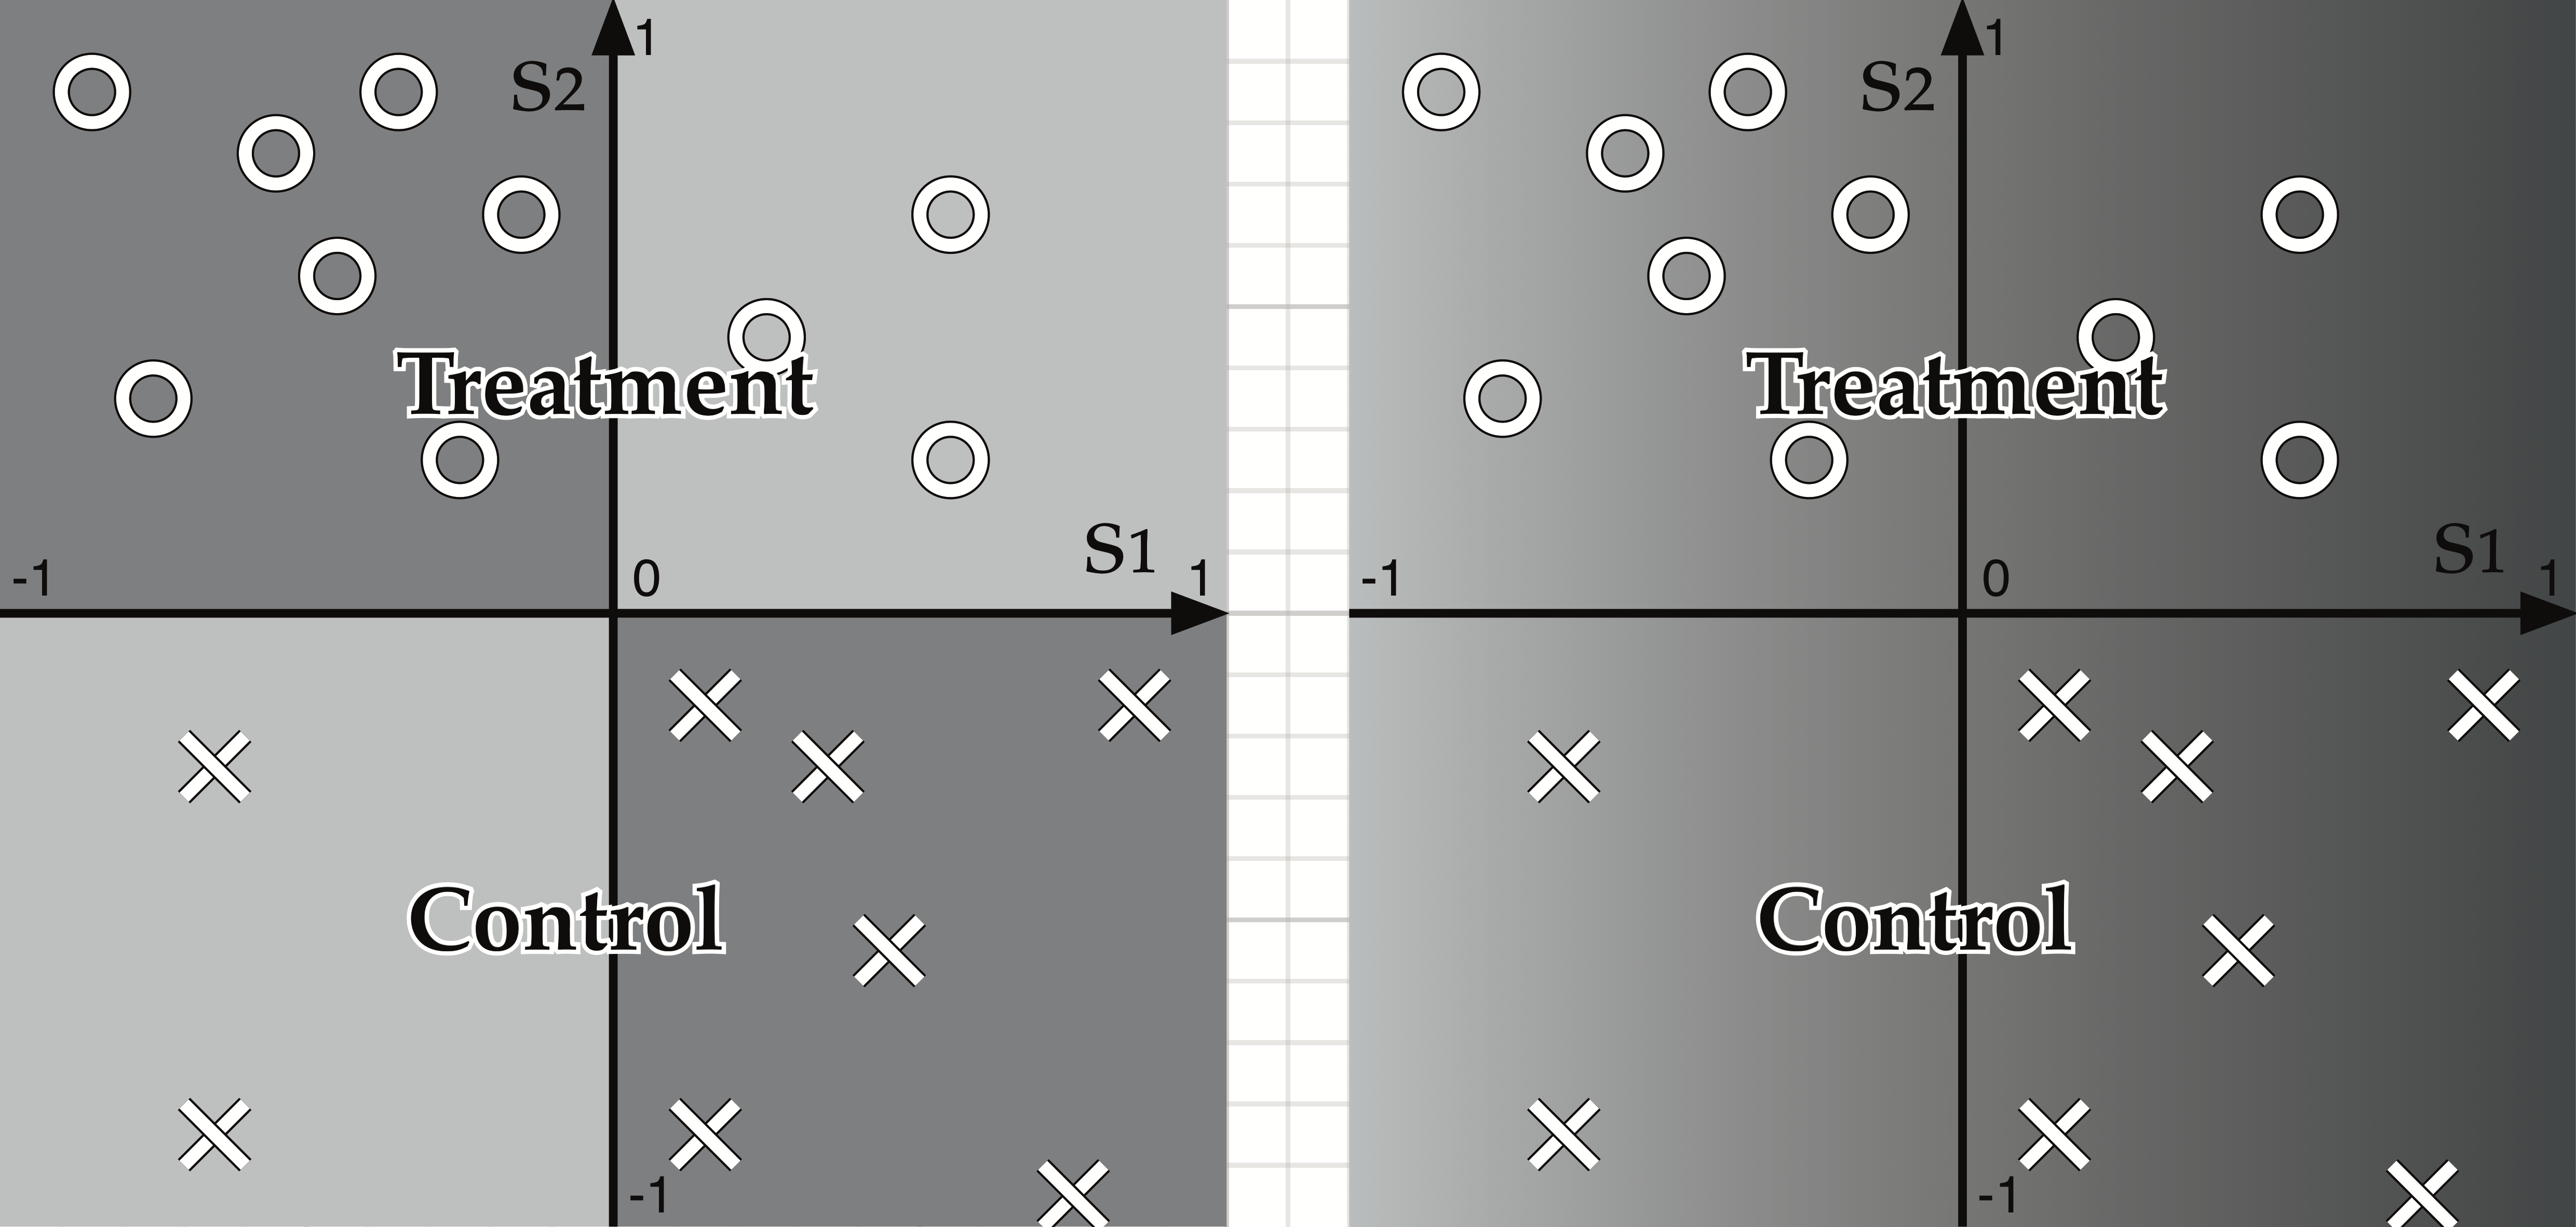
\includegraphics[height=0.35\textheight]{figures/confounding/confounding.png}
    \caption{A theoretical example illustrating the susceptibility of the projected 1D~RDD method to spatial confounding. The locations of treatment and control units are shown with circles and crosses respectively, separated by a border at \(s_2 = 0\). Units are denser in the upper left and lower right quadrants. The treatment effect, depicted as a gradient from blue to red, increases linearly with \(s_1\). \label{fig:confounding}}
\end{figure}



Suppose we have units in a 2D square, with spatial coordinates \(\svec_1 \in [-1,1]\), and \(\svec_2 \in [-1,1]\), and with a horizontal border at \(s_2=0\) separating a treatment region from a control region.
Let us assume the null hypothesis, with outcomes driven only by \(\svec_1\) (parallel to the border), given by \(Y_{i} = \alpha \svec_{1i} + \epsilon_i\),
where \(\epsilon_i\) is an iid noise term \(\epsilon_i \sim \normal\del{0, \sigman^2}\).
Lastly, let us consider the situation where the density \(\rho(\svec)\) of units is different in each quadrant of the square:
\begin{equation}
    \begin{aligned}
        \rho(\svec) = 2\rho_0 & \text{, where }\svec_1 < 0,~\svec_2 > 0 & \text{ (top left)} \\
        \rho(\svec) = \rho_0 & \text{, where }\svec_1 > 0,~\svec_2 > 0 & \text{ (top right)} \\
        \rho(\svec) = 2\rho_0 & \text{, where }\svec_1 > 0,~\svec_2 < 0 & \text{ (bottom right)}  \\
        \rho(\svec) = \rho_0 & \text{, where }\svec_1 < 0,~\svec_2 < 0 & \text{ (bottom left)}
    \end{aligned}
\end{equation}
The projection RDD then considers a 1D RDD along \(s_2\).
The usual RDD estimand \autoref*{M-eq:rdd_univ_estimand} can be obtained analytically, and equals \(\tau=\frac{-\alpha}{3}\), despite assuming the null hypothesis.
This is because \(s_1\) acts as a hidden confounder, whose distribution changes discontinuously at the border, which leads to bias and inconsistency in the projected 1D~RDD estimate.
In geographical settings, a discontinuous change in the density of units at the border is not unusual: for example a border could run alongside a park, or a small body of water, therefore with zero population density on one side of the border.
A visual inspection of \autoref*{M-fig:sales_map} showing the locations of units in a New York City property sales dataset reveals many examples of this.


\hypertarget{characterizing-and-estimating-the-average-treatment-effect}{%
\section{Characterizing and Estimating the Average Treatment Effect}
}
\hypertarget{projected-land-ate}{%
\subsection{Projected Land ATE}
}
In certain applications, population-based estimands can be undesirable, especially if the locations at which measurements are made are not representative of the population of interest.
In such cases, geography-weighted estimands can be more natural.
See \cite{antonelli2016positive} for a discussion of this distinction in the context of preferential sampling.
Remember that the ``geometry-based'' estimand \(\unifavg\) places uniform weights along the border.
Instead, the ``geography-based'' projected land ATE estimand \(\taugeo\), illustrated in \autoref{fig:mississippi_projection_methods}(b), begins by placing uniform weights on the treatment and control areas \(\area_\treat\) and \(\area_\ctrol\) that are within distance \(\buffer\) of the border \(\border\), but then projects them onto the border to derive border weights.
In other words, the projection method from \(\tauproj\) is applied to an infinite population of uniform density on both sides of the border, instead of the finite population of observed units.

We denote the border vicinity area by \(\area_\buffer\), defined as all points \(\svec\) such that \(\svec \in {\area_\treat \cup \area_\ctrol}\), and \(\dist_{\border}\del{\svec} < \buffer\).
To estimate \(\taugeo\), a tight grid \(\grid\) of evenly spaced points separated by \(\gridres\) is first generated covering \(\area_\buffer\).
Denote the number of grid points by \(L_\gridres\).
Each point \(\grid_l\), \(l=1,\dotsc,L_\gridres\) in \(\grid\) is then projected onto the border to become a sentinel.
The treatment effect at these positions is then estimated as before, yielding a mean vector and covariance matrix akin to \autoref*{M-eq:postvar2gp}.
The mean of the mean vector then gives an estimate of \(\taugeo\).
In other words, \(\taugeo\) is estimated by applying the \(\unifavg\) procedure with sentinels obtained by projecting the grid points, instead of equispaced sentinels.
\(\taugeo\) remains in the category of weighted-mean estimands, with the weight function \(\weightb(\sentinel)\) in \autoref*{M-eq:weighted_estimand} proportional to the area of \(\treatarea\) and \(\ctrolarea\) that \(\sentinel\) is nearest to, which can be written as the limit as the grid spacing goes to zero of point masses at the grid locations projected onto the border:
\begin{equation}
    \weightb(\sentinel) = \lim_{\gridres \rightarrow 0}\frac{1}{L_\gridres}\sum_{l=1}^{L_\gridres} \Ind\cbr{\sentinel = \proj_{\border}\del{\grid_l} }\,,
\end{equation}
where \(\Ind\) is the indicator function that returns one if its argument is true and zero otherwise.

For certain applications, it may be desirable to further restrict \(\area_\buffer\) to only certain types of land, for example residential areas in social studies, or farmland in agricultural studies.
However, it is important to note that \(\taugeo\) is never interpretable as the average treatment effect in the vicinity of the border, that is \(\taugeo \neq \int_{\area_\buffer} \tau(\svec) \dif \svec\).
Estimating the latter estimand would require predicting the conditional regression function at grod locations within the treatment or control region using only observations on the \emph{other} side of the border, which increases the extent of extrapolation required and thus makes the analysis more vulnerable to model misspecification.



\hypertarget{projected-super-population-ate}{%
\subsection{Projected Super-Population ATE}
}

\begin{figure}[tbp]
    \centering
    \includegraphics[width=\textwidth]{../figures/mississippi_projection_methods.png}
    \caption{\label{fig:mississippi_projection_methods}
        Illustration of (a) projected finite-population ATE \(\tauproj\), and (b) projected land ATE \(\taugeo\), using the border separating Mississippi and Louisiana near Baton Rouge, with units at the centroid of each county.
        The border vicinity \(\area_\buffer\) is defined as all land within \(\buffer=50\,\mathrm{km}\) of the border.
    With both methods, every projected sentinel has equal weight in the ATE, but the tight grid in (b) causes sentinels to coincide or nearly coincide, which we depict by scaling up the size of the marker by the number of coinciding sentinels.}
\end{figure}

Lastly, the purely geographical estimand \(\taugeo\) can be modified by weighting the grid points \(\grid_l\), \(l=1,\dotsc,L_\buffer\) by the population density \(\rho\del{\grid_l}\).
This gives the projected superpopulation ATE \(\taupop\).
Similarly to the density-weighted ATE \(\taurho\), estimating \(\taupop\) requires an estimate of the density \(\rho\del{\grid_l}\) at every grid point.
As before, the uncertainty in the estimate of \(\rho\) should in principle be propagated to the estimate of \(\taupop\), which generally will make the posterior distribution of \(\taupop\) neither normal nor analytically tractable.

The estimand \(\taupop\) can be interpreted as giving equal weight to each unit in the superpopulation of units within the border vicinity \(\area_\buffer\), but then moving each unit from its original location to its nearest location along the border, where the GeoRDD setting allows for the estimation of the treatment effect without undue extrapolation, and finally averaging the treatment effect of each unit in this displaced superpopulation.



\hypertarget{wiggly-border-simulation}{%
\subsection{Wiggly Border Simulation}
\label{sec:wiggly_border}
}
    

\begin{figure}[tbp]
\centering
\includegraphics[height=0.35\textheight]{../figures/wiggly_boundaries_setup.png}
\caption{\label{fig:wiggly_boundaries_setup}Spatial positions of units and border for the wiggly border simulation of \autoref{sec:wiggly_border}. Projection lines for the projected finite population ATE are shown in light gray.}
\end{figure}
    

        We illustrate the above ATE estimators with a simulation.
200 units are placed in a square area delimited by spatial coordinates \(S_1 \in \cbr{0,2}\) and \(S_2 \in \cbr{-1, 1}\).
A border at \(S_2=0\) divides units vertically into a control and treatment region,
which are then further divided horizontally at \(S_1=0.5\) and \(S_1=1.5\) into three bands:

\begin{itemize}
\item
  The leftmost band \(S_1 < 0.5\) has a weak treatment effect.
\item
  The middle band \(0.5 \ge S_1 < 1.5\) has a much lower population density, and a stronger treatment effect.
\item
  The rightmost band \(S_1 \ge 1.5\), has a much higher population density, and a very strong treatment effect.
\end{itemize}

Furthermore, the border in the leftmost band is a triangular wave, to create ``wiggliness.''
We increase the number of wiggles from 0 to 1000 to observe the effect on the estimates.
The simulation setting is summarized in \autoref{table:wiggly_setup}.
We draw a single set of spatial coordinates, shown in \autoref{fig:wiggly_boundaries_setup}, then draw 10,000 simulations of the outcomes \(Y\) from a Gaussian process with squared exponential kernel (\(\ell=0.4\), \(\sigma=0.5\)).
To units above the border we add a treatment effect \(\tau(S_1, S_2) = S_1\).



\begin{table}[tbp]
\centering
\begin{tabular}{llll}
\hline
& Left \(S_1< 0.5\) & Middle \(0.5 \ge S_1 < 1.5\) & Right \(1.5 \ge S_1\)\tabularnewline
\hline
\textbf{Border} & wiggly & straight & straight\tabularnewline
\textbf{Density} & low \(\rho=1.0\) & very low \(\rho=0.3\) & high \(\rho=2.0\)\tabularnewline
\(\taubold\) & weak & medium & strong\tabularnewline
\hline
\end{tabular}
\caption{Summary of wiggly border simulation setup. \label{table:wiggly_setup}}
\end{table}

        We fit the Gaussian process model \autoref*{M-eq:spec2gp},
using the known hyperparameters of the covariance kernel and a weak prior on the mean parameter of each region,
and estimate the average treatment effect using the six methods proposed above.
In \autoref{fig:wiggly_boundaries_posteriors}(a) we show, for each estimator, the corresponding estimand and average posterior mean estimate evolving as the number of border wiggles increases.
The behavior of the posterior standard deviation is shown in \autoref{fig:wiggly_boundaries_posteriors}(b).

\begin{figure}[tbp]
\centering
\includegraphics[height=0.4\textheight]{../figures/wiggly_boundaries_posteriors.png}
\caption{\label{fig:wiggly_boundaries_posteriors} Results of the simulations of \autoref{sec:wiggly_border}, showing for each ATE estimator as the leftmost section of the border gets wigglier (a) the estimate (posterior mean) averaged over 10,000 simulations with the corresponding estimand shown as a dotted line of the same color, and (b) the posterior standard deviation.}
\end{figure}
    
As the border is a straight line and \(\treatarea\) and \(\ctrolarea\) are rectangles,
and as the treatment effect does not depend on the vertical axis \(S_2\),
the density-weighted estimand \(\taurho\) equals the projected superpopulation estimand \(\taupop\),
and they are in fact both equal to the infinite-population average treatment effect.
Correspondingly, the posteriors of \(\taurho\) and \(\taupop\) are identical.
With 200 units, \(\taupop\) and the finite-population projected ATE \(\tauproj\) are also similar, but the latter has the advantage of not require estimating the population density.

The geometry- and geography-based ATE \(\unifavg\) and \(\taugeo\) are also equivalent when the border is a straight line.
They give equal weight to the sparsely populated middle band, which produces a lower estimate with higher variance than the posteriors of \(\taurho\) and \(\taupop\).

Lastly, the information-based inverse-variance estimand \(\invvar\) does not coincide with any others.
The estimand and mean estimate change slightly from 0 to 1 wiggles, but remains stable thereafter, demonstrating the robustness of this estimator to border topology.
Weighting by the inverse variance gives the lowest posterior variance within the class of ATEs under consideration, which can indeed be seen in \autoref{fig:wiggly_boundaries_posteriors}(b).

As we introduce wiggles into the leftmost band,
\(\taurho\) and \(\unifavg\) show their susceptibility to the border topology.
Proportionally more sentinels are packed into the leftmost section of the border,
upweighting the lower treatment effect of that band,
and resulting in a drop of the two estimates and estimands.
Meanwhile, \(\invvar\) remains stable despite the wiggles,
because the additional sentinels in the leftmost
band get automatically downweighted as their correlation rises.
The estimators that rely on projection
\(\tauproj\), \(\taugeo\), and \(\taupop\) also remain stable,
because the projected sentinels hardly move.
These robust estimands show only a slight displacement when the first wiggles are introduced,
caused by the presence of some sentinels nearer to the observed units.
    
\begin{figure}[ptb]
\centering
\includegraphics[width=\textwidth]{../figures/weight_functions.png}
\caption{\label{fig:weight_functions}Weight functions and induced weights on the observations for the six weight functions proposed in this paper. The weight function plots show the weight \(\weightb(\sentinel)\) against each sentinel's \(S_1\) coordinate. Sentinels with coinciding or nearly coinciding (within 0.005 of each other) coordinate \(S_1\) were merged and their weights summed. The induced weight plots show a circle for each unit, with the area of the circle proportional to its weight (\(\wt\) and \(\wc\) for treatment and control units respectively), and colored in blue for positive weights and orange for negative weights.}
\end{figure}
    

        In \autoref{fig:weight_functions}(a-f), we illustrate the behavior of border weights \(\weightb(\sentinel)\) and unit weights (\(\wt\) and \(\wc\)) in this simulation setting with 3 wiggles.
Note how evenly spaced sentinels (for \(\unifavg\), \(\taurho\), and \(\invvar\)) are more densely packed along \(S_1\) in the leftmost area because of the zig-zagging border.
The inverse-variance weighted estimator border weights can be seen to respond to this change in the border topology, though it is difficult to interpret their oscillating behavior.
While these border-weights look unreasonable and unstable, the induced unit weights for \(\invvar\) are well-behaved, and in fact quite similar to those of the projected finite- and infinite-population estimators.
Furthermore, note that all estimators can give some small negative weights \(\wt\) to treatment units, and small positive weights \(\wc\) to control units.
For Gaussian processes, this can be understood in terms of the negative side-lobes of the equivalent kernel (see \cite{rasmussen2006gaussian} Section 2.6).
The high variance of \(\unifavg\) and \(\taugeo\) manifests itself as large weights given to a small number of units.
All other estimators spread the weights more evenly amongst the units near the border, which reduces their variance.
    


        For comparison, the weights placed on units by the projected 1D RDD are shown in \autoref{fig:weight_functions}(g).
A triangular kernel in \(S_2\) was used with bandwidth selected using the MSE-minimizing method proposed by \cite{imbens2012optimal}.
The Projected 1D~RDD estimator can also be written as a linear combination of the observed outcomes \autoref*{M-eq:unit_weights}, and the unit weight vectors can be derived as:
\begin{equation}
\begin{split}
\wt &= \hphantom{-} \Xmat_b (\Xmat_\treat\trans \Wmat_\treat \Xmat_\treat)^{-1} \Xmat_\treat\trans \Wmat_\treat \,, 
\text{ and}
\\
\wc &= - \Xmat_b (\Xmat_\ctrol\trans \Wmat_\ctrol \Xmat_\ctrol)^{-1} \Xmat_\ctrol\trans \Wmat_\ctrol \,, 
\end{split}
\label{eq:unit_weights_llr}
\end{equation}
where \(\Xmat_b = \del{1~0}\), \(\Xmat_\treat\) is the \(n_\treat \times 2\) design matrix with the first column filled with ones and the second column containing the distance from the border of each treatment unit, and \(\Wmat_\treat\) is an \(n_\treat \times n_\treat\) diagonal matrix where the \(i^\mathrm{th}\) diagonal element is the triangular kernel evaluated on the \(i^\mathrm{th}\) unit's distance from the border.
The \(\Xmat_\ctrol\) and \(\Wmat_\ctrol\) matrices are analogously defined for control units.
By construction, the unit weights drop to zero outside of the support of the kernel.
Within the support, Projected 1D RDD can also give negative weights to treatment units, and positive weights to control units.
This results from the negative influence on the prediction \(\widehat{y^*}\) at \(x^*\) that univariate linear regression can give to an observation \(Y_i\) at \(X_i\) sufficiently far away on the opposite side of the mean \(\overline{X}\) of all observations.
Strikingly, almost all of the positive weights are given to units in the rightmost treatment area that are closest to the border, and almost all the negative weights are given to units in the leftmost control area.
Consequently, any trend in the outcomes across \(S_1\) would confound the estimated treatment effect.

\hypertarget{testing-for-non-zero-effect}{%
\section{Testing for Non-Zero Effect}
\label{sec:hypothesis_testing}
}

\hypertarget{marginal-likelihood-test}{%
\subsection{Marginal Likelihood Test}
}

To target the sharp null hypothesis, we first define a parametric null model \(\modnull\),
specified as a single Gaussian process spanning the control and treatment regions,
with the same kernel and hyperparameters obtained in the 2GP procedure.
\(\modnull\) is smooth and continuous at the border,
and therefore accords with the sharp null hypothesis.
Intuitively, if there is a treatment effect,
the likelihood of the observations should be lower under \(\modnull\) than under \(\modalt\),
the \(\GP\) model as specified in \autoref*{M-eq:spec2gp}.
We therefore choose the difference in log-likelihoods as our test statistic
\begin{equation}
    t = \log \Pr\del{\yt{}, \yc{} \mid \modalt} - \log \Pr\del{\yt{}, \yc{} \mid \modnull} \,,
\end{equation}
and wish to reject the sharp null hypothesis when its observed value \(t_{obs}\) is high.

A parametric bootstrap approach is used to quantify what ``high'' means. We draw \(\yt{}^*,\yc{}^*\) from \(\modnull\),
using the same spatial locations as in the original data,
and then fit the two competing models to the simulated data in order to obtain the bootstrapped test statistic
\begin{equation}
    t^* = \log \Pr\del{\yt{}^*, \yc{}^* \mid \modalt} - \log \Pr\del{\yt{}^*, \yc{}^* \mid \modnull}\,.
\end{equation}
Repeating this procedure, we obtain a distribution of \(t\) under \(\modnull\),
which we can then compare to the observed \(t\).
More precisely, we can interpret the proportion of \(t^*\) drawn above \(t_{obs}\) as a \(p\)-value
\begin{equation}
    p^{\mathrm{lik}} = \Pr\del{t^* > t_{obs} \mid \modnull}\,.
\end{equation}
Computationally, because the hyperparameters and locations of the units are held constant during the bootstrap, we can reuse the Cholesky decomposition of the covariance matrix, allowing the test to be performed in seconds even with hundreds of units and thousands of bootstrap samples.



\hypertarget{chi-squared-test}{%
\subsection{``Chi-squared'' Test}
}
The likelihood-based sharp null above is valid and easy to understand.
But it may seem odd that the test aims to detect a non-zero treatment effect at the border, without any explicit reference to the border \(\border\).
The test statistic and \(p\)-values can be computed without access to the sentinel positions, using only the treatment and control indicators.
If the test is significant, there is no guarantee that this is due to a discontinuity at the border.

To address this oddity, we can derive a test statistic directly from the cliff face estimator \autoref*{M-eq:postvar2gp}.
We will use \(\muvec\) and \(\SigmaMat\) as shorthand for the posterior mean \(\muvec_{\sentinels \mid Y}\)
and covariance matrix \(\SigmaMat_{\sentinels \mid Y}\) throughout this section.
If a \(k\)-vector \(\yvec\) is distributed \(\normal\del{\muvec, \Sigma}\), with mean vector \(\muvec\) unknown and covariance \(\SigmaMat\) known, then under the null hypothesis that \(\mu=0\), the test statistic \(\yvec\trans \SigmaMat^{-1} \yvec\) has distribution \(\chi^2_k\).
See for example \cite{rencher2003methods} Section 5.2.2 for a classical derivation of this test.
This suggests that we could use \(S^2=\muvec\trans \SigmaMat^{-1} \muvec\) as a test statistic,
and obtain a \(p\)-value from a \(\chi^2_\numsent\) distribution function evaluated at \(S^2\), where \(\numsent\) is the number of sentinels.
However, we face two problems.
Firstly, this test, obtained heuristically from a Bayesian posterior by analogy with the classical multivariate normal result, is not a valid frequentist test.
Secondly, while \(\SigmaMat\) is mathematically full-rank, it is typically numerically rank-deficient.
Therefore, \(\numsent\) overestimates the true degrees of freedom of the null distribution.

Benavoli and Mangili (2015), developing a test for function equality, address the second problem by trimming the \(\SigmaMat\) eigenvalues \(\lambda_i\) lower than \(\epsilon \sum_{j=1}^k \lambda_j\), with \(\epsilon\) a pre-specified small number (they use 0.01).
They address the first problem by showing that the resulting \(p\)-value is always conservative in their simulations.
However, in our work, we found the resulting \(p\)-value to be sensitive to the arbitrarily chosen \(\epsilon\) tolerance parameter, which makes it difficult to trust its validity.

We therefore again take the parametric bootstrap approach, this time using \(S^2\) as the test statistic instead of the likelihood ratio.
With B bootstrap samples, the \(p\)-value is obtained as
\begin{equation}
    \begin{split}
        p &= \frac{1}{B} \sum_{t=1}^T \Ind\cbr{S_{(b)}^2 < S^2}\  \text{, with}\\
        S_{(b)}^2 &= (\muvec_{(b)} )\trans \SigmaMat^{-1} \muvec_{(b)}\,,
    \end{split}
\end{equation}
where \(\muvec_{(b)}\) is the result of applying \autoref*{M-eq:postvar2gp} to \(\yt^{(b)}\) and \(\yc^{(b)}\), themselves drawn from \(\modnull\) at the same locations as the observations \(\yt\) and \(\yc\).

Because calculating \(S^2\) involves inverting a matrix \(\Sigma\) that is mathematically of full rank, but numerically of low rank, we may worry about the numerical stability of computing \(S\).
We verified in simulated examples that regularizing \(\Sigma\) by adding a small constant to its diagonal does not greatly affect the computed \(S^2\).
The parametric bootstrap ensures the frequentist validity of the test
regardless of the regularization.


\hypertarget{power-in-simulated-example}{%
\subsection{Power in Simulated Example}
\label{sec:powersim}
}



\begin{figure}[tbp]
    \centering
    \includegraphics[height=0.4\textheight]{../figures/mississippi_sim.png}
    \caption{\label{fig:mississippi_counties}Set-up of the imaginary experiment in Louisiana and Mississippi. Each unit is at the centroid of a county. The colors indicated the observed outcomes in one draw of the simulation under \(\tau=1.5\). In this particular run, the p-values were 0.0016, 0.0018, and 0.0013 for the mLL, \(\chi^2\), and inverse-variance test respectively.}
\end{figure}



The three tests we developed leverage different aspects of the problem, and target two different null hypotheses. One may wonder how their power compares in the presence of a treatment effect. Considering once more the border between Louisiana and Mississippi, we imagine an experiment where the unit of analysis is the county, located at its centroid, as shown in \autoref{fig:mississippi_counties}.
We will simulate outcomes from a single Gaussian process covering both states. For simplicity, we fix the hyperparameters to arbitrary values: \(\sigman=\sigmaf=1.0\) and \(\ell=100\,\mathrm{km}\).
We then add a constant treatment effect \(\tau\) to all the outcomes in Louisiana.
The results of the three tests proposed so far are shown in the first three rows of \autoref{table:power} for \(\tau=0\) (null hypothesis) and \(\tau=1.2\) and significance level \(\alpha=0.05\).


\begin{table}
    \label{table:power}
    \centering
    \begin{tabular}{rrr}
        \hline
        & \multicolumn{2}{c}{Power under} \\
        Test & $\tau=0$ & $\tau=1.2$ \\
        \hline
        Marginal log-likelihood $ $ & 0.048 & 0.656 \\
        $\chi^2$ & 0.047 & 0.635 \\
        Inverse-variance $\Sigma^{-1}$ & 0.085 & 0.866 \\
        Bootstrap-calibrated $\Sigma^{-1}$ & 0.050 & 0.799 \\
        Analytically calibrated $\Sigma^{-1}$ & 0.051 & 0.801 \\
        \hline
    \end{tabular}
    \caption{Power of marginal likelihood, chi-squared, and inverse-variance tests, with nominal significance of $\alpha=0.05$, under null and alternative hypothesis for simulated outcomes at the centroids of Louisiana and Mississippi counties.}
\end{table}
We see that under the null, the \(\chi^2\) and likelihood ratio tests are valid (rejection of the null in 5\% of simulations up to simulation error).
This is enforced by the parametric bootstrap, which draws test statistics from the same null distribution to calibrate the tests.
However, the \(p\)-values for the inverse-variance test are biased down, so that we will falsely reject the null \(6.7\%\) instead of \(5\%\) of the time.
While unfortunate, this is unsurprising, since the inverse-variance test was derived heuristically rather than from a rigorous frequentist procedure.

After calibration, the hypothesis test based on the inverse-variance mean is valid, but retains higher power to detect the constant treatment effect than the mLL and \(\chi^2\) tests.
This can lead to a paradox: we may reject the weak null hypothesis, but fail to reject the sharp null hypothesis (using the \(\chi^2\) or likelihood test), even though rejection of the weak null logically implies rejection of the sharp null.
This paradox isn't specific to this setting, and is discussed in depth in the context of randomization-based inference by \cite{Ding:2014sf}.
To maximize power, we therefore recommend using the calibrated inverse-variance test in studies where the main interest is in the detection of an overall (average) increase or decrease in outcomes.


%%% NYC %%%
\hypertarget{application-nyc-school-districts}{%
\section{Application: NYC School Districts}
\label{sec:NYC_example}
}

\hypertarget{nyc-hypothesis-tests}{%
\subsection{Additional Hypothesis Tests}\label{sec:nyc_hypothesis_tests}}

\begin{table}[tbp]
    \centering
    \label{table:NYC_tests}
    \begin{tabular}{ll}
        \hline
        Test                   & $p$-value \\
        \hline
        $\chi^2$ bootstrap     & 0.012     \\
        mLL bootstrap          & 0.002     \\
        $\invvar$ uncalibrated & 0.0007    \\
        $\invvar$ calibrated   & 0.002 \\
        \hline
    \end{tabular}
    \caption{Results of hypothesis tests for New York school district house prices.}
\end{table}

To assess the validity of the three tests, we apply the placebo tests devised in \autoref*{M-sec:placebo}.
Within each district, we split the data in half by a line at angles \(1\degree\), \(3\degree\), \(5\degree\), \(6\degree\), \(\dotsc\), \(179\degree\).
Because these lines were drawn arbitrarily, we don't expect a discontinuous treatment effect between the two halves, and so we hope to see a uniform distribution of placebo \(p\)-values.
However, these tests will be highly correlated,
and so the low effective sample size could lead to some apparent departures from uniformity.
There is in fact visible autocorrelation in the graphs of placebo \(p\)-values as a function of angle.

\begin{figure}[tbp]
    \centering
    \includegraphics[width=\textwidth]{../NYC/NYC_plots/NYC_placebos.png}
    \caption{\label{fig:nyc_placebos} Placebo tests for significance tests applied to NYC school district house prices, applied within districts 19 and 27. The three rows respectively show results for the marginal log-likelihood bootstrap test, chi-squared bootrap test, and calibrated inverse-variance test. The first column shows the placebo p-value as a function of the border angle; the second column shows histograms of the placebo p-values, with the black vertical line indicating the uniform distribution.}
\end{figure}

The mLL placebo \(p\)-values show a pronounced bias towards low values.
This seems to confirm our concern that the marginal log-likelihood may be sensitive to features of the data other than the discontinuity at the border.
In particular, model misspecification, which is a concern in spatial models, makes the interpretation of the mLL test unreliable.
Based on this vulnerability, and its manifestation in this application, we do not recommend relying on the likelihood-ratio test.

The \(\chi^2\) test shows more robustness, with \autoref{fig:nyc_placebos}(d) showing some negative bias in district 27, and some positive bias in district 19, which could simply be due to the low effective sample size.
We therefore believe that the \(\chi^2\) test will continue to be reliable under misspecification.
It is only due to its low power that we hesitate to recommend its use in applications where the treatment effect is expected to be fairly homogenous.

Lastly, the calibrated inverse-variance placebo \(p\)-values display no obvious bias, with \autoref{fig:nyc_placebos}(f) close to uniformly distributed, and \autoref{fig:nyc_placebos}(e) showing a lower auto-correlation than the mLL and \(\chi^2\) tests.
The high power and robustness of the inverse-variance test make a strong case for its use in most applications.

\hypertarget{pairs-of-school-districts}{%
\subsection{Pairs of School Districts}\label{pairs-of-school-districts}}



The GeoRDD analysis can be repeated for each pair of adjacent districts.
\autoref{fig:NYC_pairwise} and \autoref{table:NYC_pairwise} give an overview of the results by showing the posterior mean and standard deviation of the inverse variance ATE estimated at each border.
Significant effects are found between many districts, but interpreting the results requires some caution.
We have already mentioned the issue of compound treatments for borders between school districts that overlap with the border between boroughs.
School districts 19, 32, and 14 are in Brooklyn, while districts 30, 24, and 27 are in Queens.


\begin{figure}[tbp]
    \centering
    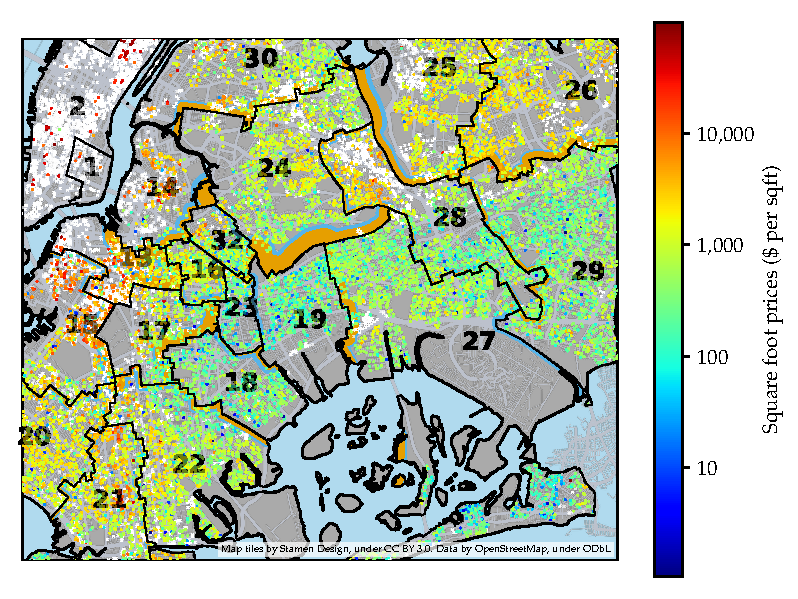
\includegraphics[width=\textwidth,height=0.8\textheight,keepaspectratio]{../NYC/NYC_plots/pairwise_mean_se.png}
    \caption{\label{fig:NYC_pairwise}
        Pairwise estimates of the inverse variance ATE between adjacent districts.
        The thickness of the orange buffer adjacent to borders is proportional to the posterior mean of the inverse variance ATE, and the blue buffer beyond it is proportional to the posterior standard deviation of the ATE.
    The buffers are drawn on the side of the border that is estimated to have higher house prices.}
\end{figure}

Some school districts are separated by parks (or other non-residential zones), for example districts 15 \& 17 or 19 \& 24, so that house sales do not extend all the way to the border on one or both sides.
A significant treatment effect between these pairs cannot be interpreted as the detection of a discontinuity in prices at the border, let alone any kind of causal interpretation, but rather it means that the difference in prices between the two sides of the park exceeds the typical spatial variation of house prices expected over the same distance.
This is not unsurprising, and one may speculate that physical barriers like parks, rivers, railways and major roads can separate neighborhoods with distinct character, demographics and thus house prices.
This in turn challenges the stationarity assumption of the spatial model \autoref*{M-eq:spec2gp}.
The higher distance between data and the border also stretches the spatial model's ability to extrapolate, which makes it more vulnerable to model misspecification.

Other pairs of district, like 13 \& 14, 13 \& 17, and 25 \& 28 have clusters of missing data (condo sales with unknown square footage) near the border that cast doubt on the interpretation of the estimated effect.
Nonetheless, significant effects are also found between pairs of school districts without issues due to compound treatments, physical barriers, or missing data.
House prices increase going across the border from districts 16 to 13, 18 to 17, 24 to 30, 23 to 17, 25 to 26, 28 to 29, and 29 to 26.
Overall, it seems that school district borders in Brooklyn and Queens can correspond to measurable jumps in house prices per square foot.
The estimated size of this effect varies: zero or negligible in some cases, such as between districts 15, 20, 21, and 22; and quite pronounced in others, such as a 20\% price increase from 29 to 26, or 22\% from 18 to 17.


%%% TABLES %%%

\newgeometry{margin=2cm} % modify this if you need even more space
\begin{landscape}

\hypertarget{tables}{%
\section{Tables}
\label{sec:tables}
}

    \begin{table}[!h]
        \begin{tabular}{r|rrrrrrrrrrrr}
            \hline
            $n_{\mathrm{wiggles}}$ & $\widehat{\unifavg}$ & $\unifavg$ & $\widehat{\invvar}$ & $\invvar$ & $\widehat{\taurho}$ & $\taurho$ & $\widehat{\tauproj}$ & $\tauproj$ & $\widehat{\taugeo}$ & $\taugeo$ & $\widehat{\taupop}$ & $\taupop$\\
            \hline
            0        & 1.02 (0.14) & 1.00    & 1.23 (0.10) & 1.23   & 1.21 (0.10) & 1.21   & 1.23 (0.10) & 1.24    & 1.02 (0.14) & 1.00   & 1.21 (0.10) & 1.21   \\
            1        & 1.01 (0.13) & 0.99    & 1.14 (0.09) & 1.16   & 1.19 (0.10) & 1.19   & 1.24 (0.10) & 1.24    & 0.99 (0.13) & 0.97   & 1.17 (0.10) & 1.17   \\
            2        & 0.98 (0.13) & 0.95    & 1.14 (0.09) & 1.16   & 1.15 (0.10) & 1.14   & 1.24 (0.10) & 1.24    & 0.97 (0.13) & 0.94   & 1.14 (0.10) & 1.14   \\
            3        & 0.94 (0.13) & 0.91    & 1.14 (0.09) & 1.16   & 1.09 (0.10) & 1.08   & 1.23 (0.10) & 1.23    & 0.96 (0.13) & 0.93   & 1.13 (0.10) & 1.12   \\
            5        & 0.86 (0.13) & 0.82    & 1.14 (0.09) & 1.15   & 0.98 (0.11) & 0.96   & 1.23 (0.10) & 1.23    & 0.95 (0.13) & 0.92   & 1.12 (0.10) & 1.11   \\
            10       & 0.72 (0.14) & 0.67    & 1.14 (0.09) & 1.15   & 0.80 (0.13) & 0.76   & 1.23 (0.10) & 1.23    & 0.95 (0.13) & 0.92   & 1.12 (0.10) & 1.11   \\
            20       & 0.58 (0.15) & 0.52    & 1.14 (0.09) & 1.15   & 0.63 (0.14) & 0.58   & 1.23 (0.10) & 1.23    & 0.95 (0.13) & 0.92   & 1.12 (0.10) & 1.11   \\
            40       & 0.48 (0.16) & 0.41    & 1.14 (0.09) & 1.15   & 0.50 (0.16) & 0.44   & 1.23 (0.10) & 1.23    & 0.95 (0.13) & 0.92   & 1.12 (0.10) & 1.11   \\
            80       & 0.41 (0.17) & 0.34    & 1.14 (0.09) & 1.15   & 0.42 (0.17) & 0.35   & 1.23 (0.10) & 1.23    & 0.95 (0.13) & 0.92   & 1.12 (0.10) & 1.11   \\
            160      & 0.37 (0.18) & 0.30    & 1.14 (0.09) & 1.15   & 0.38 (0.18) & 0.30   & 1.23 (0.10) & 1.23    & 0.94 (0.13) & 0.92   & 1.11 (0.10) & 1.11   \\
            320      & 0.36 (0.18) & 0.27    & 1.14 (0.09) & 1.15   & 0.36 (0.18) & 0.28   & 1.23 (0.10) & 1.23    & 0.95 (0.13) & 0.92   & 1.12 (0.10) & 1.11   \\
            640      & 0.34 (0.18) & 0.26    & 1.14 (0.09) & 1.15   & 0.35 (0.18) & 0.26   & 1.24 (0.10) & 1.23    & 0.95 (0.13) & 0.92   & 1.12 (0.10) & 1.11   \\
            1000     & 0.35 (0.18) & 0.26    & 1.15 (0.09) & 1.15   & 0.35 (0.18) & 0.26   & 1.24 (0.10) & 1.23    & 0.95 (0.13) & 0.92   & 1.12 (0.10) & 1.11 
            \\    \hline
        \end{tabular}
        \caption{\textbf{Wiggly Border Simulation Results} Posterior mean averaged over 10,000 simulations, posterior standard deviation and true value for each average treatment effect estimand as the wiggliness of the border is increased in the simulations of \autoref{sec:wiggly_border}.}
    \end{table}

    \begin{table}[!h]
        \footnotesize
        \begin{tabular}{r|lllllll}
            \hline
            \( \mathbf{13} \)& \( \mathbf{14:}~-0.29 \pm 0.09 \)& \( \mathbf{15:}~+0.03 \pm 0.07 \)& \( \mathbf{16:}~-0.13 \pm 0.07 \)& \( \mathbf{17:}~-0.26 \pm 0.08 \)\\ 
            \( \mathbf{14} \)& \( \mathbf{13:}~+0.29 \pm 0.09 \)& \( \mathbf{16:}~-0.16 \pm 0.10 \)& \( \mathbf{24:}~-0.38 \pm 0.15 \)& \( \mathbf{32:}~-0.07 \pm 0.12 \)\\ 
            \( \mathbf{15} \)& \( \mathbf{13:}~-0.03 \pm 0.07 \)& \( \mathbf{17:}~-0.18 \pm 0.10 \)& \( \mathbf{20:}~+0.05 \pm 0.06 \)& \( \mathbf{22:}~+0.24 \pm 0.11 \)\\ 
            \( \mathbf{16} \)& \( \mathbf{13:}~+0.13 \pm 0.07 \)& \( \mathbf{14:}~+0.16 \pm 0.10 \)& \( \mathbf{17:}~-0.04 \pm 0.07 \)& \( \mathbf{23:}~-0.10 \pm 0.07 \)& \( \mathbf{32:}~+0.05 \pm 0.06 \)\\ 
            \( \mathbf{17} \)& \( \mathbf{13:}~+0.26 \pm 0.08 \)& \( \mathbf{15:}~+0.18 \pm 0.10 \)& \( \mathbf{16:}~+0.04 \pm 0.07 \)& \( \mathbf{18:}~-0.20 \pm 0.07 \)& \( \mathbf{22:}~+0.06 \pm 0.07 \)& \( \mathbf{23:}~-0.29 \pm 0.10 \)\\ 
            \( \mathbf{18} \)& \( \mathbf{17:}~+0.20 \pm 0.07 \)& \( \mathbf{19:}~-0.06 \pm 0.12 \)& \( \mathbf{22:}~+0.10 \pm 0.07 \)& \( \mathbf{23:}~-0.03 \pm 0.09 \)\\ 
            \( \mathbf{19} \)& \( \mathbf{18:}~+0.06 \pm 0.12 \)& \( \mathbf{23:}~-0.00 \pm 0.08 \)& \( \mathbf{24:}~+0.39 \pm 0.11 \)& \( \mathbf{27:}~+0.19 \pm 0.06 \)& \( \mathbf{32:}~+0.27 \pm 0.12 \)\\ 
            \( \mathbf{20} \)& \( \mathbf{15:}~-0.05 \pm 0.06 \)& \( \mathbf{21:}~+0.04 \pm 0.05 \)& \( \mathbf{22:}~-0.11 \pm 0.08 \)\\ 
            \( \mathbf{21} \)& \( \mathbf{20:}~-0.04 \pm 0.05 \)& \( \mathbf{22:}~-0.04 \pm 0.05 \)\\ 
            \( \mathbf{22} \)& \( \mathbf{15:}~-0.24 \pm 0.11 \)& \( \mathbf{17:}~-0.06 \pm 0.07 \)& \( \mathbf{18:}~-0.10 \pm 0.07 \)& \( \mathbf{20:}~+0.11 \pm 0.08 \)& \( \mathbf{21:}~+0.04 \pm 0.05 \)\\ 
            \( \mathbf{23} \)& \( \mathbf{16:}~+0.10 \pm 0.07 \)& \( \mathbf{17:}~+0.29 \pm 0.10 \)& \( \mathbf{18:}~+0.03 \pm 0.09 \)& \( \mathbf{19:}~+0.00 \pm 0.08 \)& \( \mathbf{32:}~-0.04 \pm 0.08 \)\\ 
            \( \mathbf{24} \)& \( \mathbf{14:}~+0.38 \pm 0.15 \)& \( \mathbf{19:}~-0.39 \pm 0.11 \)& \( \mathbf{25:}~+0.25 \pm 0.13 \)& \( \mathbf{27:}~-0.22 \pm 0.10 \)& \( \mathbf{28:}~+0.06 \pm 0.06 \)& \( \mathbf{30:}~+0.14 \pm 0.05 \)& \( \mathbf{32:}~+0.02 \pm 0.08 \)\\ 
            \( \mathbf{25} \)& \( \mathbf{24:}~-0.25 \pm 0.13 \)& \( \mathbf{26:}~+0.08 \pm 0.04 \)& \( \mathbf{28:}~-0.15 \pm 0.08 \)& \( \mathbf{29:}~-0.06 \pm 0.10 \)& \( \mathbf{30:}~-0.28 \pm 0.15 \)\\ 
            \( \mathbf{26} \)& \( \mathbf{25:}~-0.08 \pm 0.04 \)& \( \mathbf{29:}~-0.18 \pm 0.05 \)\\ 
            \( \mathbf{27} \)& \( \mathbf{19:}~-0.19 \pm 0.06 \)& \( \mathbf{24:}~+0.22 \pm 0.10 \)& \( \mathbf{28:}~+0.04 \pm 0.04 \)& \( \mathbf{29:}~-0.01 \pm 0.08 \)\\ 
            \( \mathbf{28} \)& \( \mathbf{24:}~-0.06 \pm 0.06 \)& \( \mathbf{25:}~+0.15 \pm 0.08 \)& \( \mathbf{27:}~-0.04 \pm 0.04 \)& \( \mathbf{29:}~+0.09 \pm 0.04 \)\\ 
            \( \mathbf{29} \)& \( \mathbf{25:}~+0.06 \pm 0.10 \)& \( \mathbf{26:}~+0.18 \pm 0.05 \)& \( \mathbf{27:}~+0.01 \pm 0.08 \)& \( \mathbf{28:}~-0.09 \pm 0.04 \)\\ 
            \( \mathbf{30} \)& \( \mathbf{24:}~-0.14 \pm 0.05 \)& \( \mathbf{25:}~+0.28 \pm 0.15 \)\\ 
            \( \mathbf{32} \)& \( \mathbf{14:}~+0.07 \pm 0.12 \)& \( \mathbf{16:}~-0.05 \pm 0.06 \)& \( \mathbf{19:}~-0.27 \pm 0.12 \)& \( \mathbf{23:}~+0.04 \pm 0.08 \)& \( \mathbf{24:}~-0.02 \pm 0.08 \) \\
            \hline
        \end{tabular}
        \caption{
            \label{table:NYC_pairwise}
            \textbf{Estimated Treatment Effects Between Adjacent NYC School Districts}
            Posterior inverse variance ATE ($\pm$ posterior standard deviation) for pairs of school districts in NYC.
            Each row gives the posterior (mean $\pm$ standard deviation) of the inverse-variance ATEs for one district (row header) compared to its neighbors.
            For example the first cell indicates an estimated average change difference log house prices per square foot going from district 13 to 14 of -0.29.
        }
    \end{table}\end{landscape}
    \restoregeometry

\bibliographystyle{chicago}
\bibliography{GeoRDD}

\end{document}
